\documentclass[11pt]{article}
\usepackage[margin=1in]{geometry}
\usepackage{amsmath,amssymb,amsfonts}
\usepackage{graphicx,float}
\usepackage{fancyhdr,booktabs}
\usepackage{listings}
\usepackage{hyperref}
\usepackage{listings}
\lstset{
    language=Matlab,
    basicstyle=\ttfamily\small,
    breaklines=true,
    keepspaces=true,
    showstringspaces=false
}
\setlength{\parindent}{0pt}

\usepackage{enumitem}
\setlist[itemize,1]{label=$\bullet$}
\setlist[itemize,2]{label=$\circ$}
\setlist[itemize,3]{label=$\cdot$}
\usepackage{parskip} % Auto-manages paragraph spacing and removes indentations
\usepackage{siunitx}  % Eases typesetting of numbers and units

% US customary units
\DeclareSIUnit{\inch}{in}
\DeclareSIUnit{\foot}{ft}
\DeclareSIUnit{\yard}{yd}
\DeclareSIUnit{\mile}{mi}

\DeclareSIUnit{\slug}{slug}
\DeclareSIUnit{\lbm}{lbm}
\DeclareSIUnit{\lbf}{lbf}

\DeclareSIUnit{\psi}{psi}
\DeclareSIUnit{\psf}{psf}

\DeclareSIUnit{\gallon}{gal}
\DeclareSIUnit{\quart}{qt}
\DeclareSIUnit{\fahrenheit}{F}
\DeclareSIUnit{\rankine}{R}
\sisetup{
    per-mode = fraction
}
\usepackage{soul}
\usepackage{mathrsfs}

\geometry{margin=1in}

% Uppercase Volume with thicker, higher line
\newcommand{\vol}{\mathord{\text{\ooalign{\hidewidth $V$\hidewidth\cr\kern-0.5pt\raisebox{0.8ex}{\rule[0pt]{1em}{0.5pt}}}}}}

% Lowercase Volume with built-in shifts
\newcommand{\svol}{%
  \mathord{\text{\ooalign{%
    \hfil$v$\hfil\cr
    \hfil\rule[0.6ex]{0.8em}{0.5pt}\hfil
  }}}%
}


% Header and Footer Setup
\pagestyle{fancy}
\fancyhf{}
\lhead{ESC 340 -- Fall 2026}
\rhead{Project: Lifting Diffuser Optimization}
\cfoot{\thepage}

\title{\textbf{ESC 340 Project}\\[0.5ex]\Large Lifting Diffuser Optimization}
\author{Zeshui Song}
\date{Fall 2026}

\begin{document}
\maketitle
\vspace{-1em}

\section*{Overview}
For our project we have chosen to redesign and analyze the lifting diffuser. Our new design will optimize lifting force (pressure difference produced) compared to the basic diffuser model, and result in a more efficient device. We plan on using CAD to design and prototype possible diffuser variations and to analyze a new mathematical model for this design.\\\\
We will explore two designs: 
\begin{itemize}
    \item \textbf{Constant-gap lifting diffuser:} Optimizing the geometry of a lifting diffuser with a central air inlet and a constant gap between the diffuser and surface, similar to the design shown in class. We will analyze how parameters such as gap height, inlet diameter, and diffuser radius impact the resulting pressure distribution. Potentially use non-dimensionalization to reduce the number of parameters to optimize. 
    \item \textbf{Vortex-based lifting diffuser:} developing a model for a lifting diffuser that uses a circumferential velocity air flow in addition to radial flow to improve the pressure difference. 
\end{itemize}
\section*{Constant Gap Lifting Diffuser}
\begin{center}
    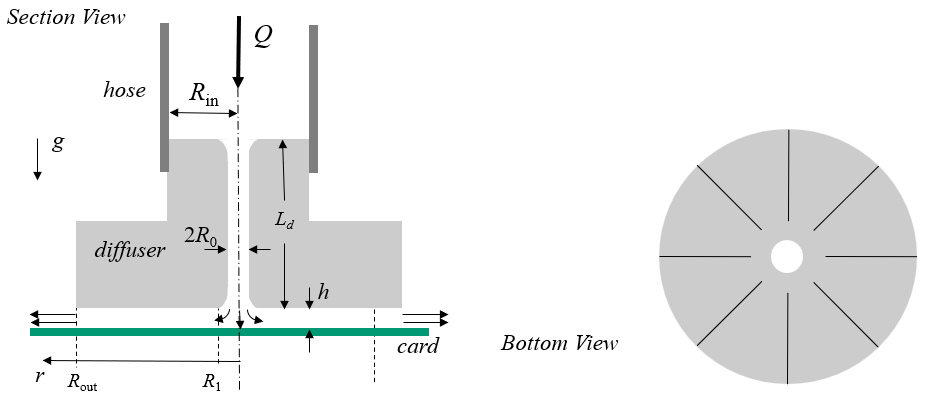
\includegraphics[width=0.9\textwidth]{constant gap.png}
\end{center}
\subsection*{Define Geometry}
\begin{itemize}
    \item $R_\text{in}$: radius of the air inlet
    \item $R_0$: radius of the central nozzle inlet
    \item $R_1$: radius of the central nozzle outlet (where the air flow enters the gap)
    \item $R_\text{out}$: outer radius of the diffuser
    \item $L_d$: length of the central nozzle
    \item $h$: gap height between the diffuser and the surface
    \item $r$: radial distance from the center of the diffuser
\end{itemize}
\subsection*{Approach}
There are two main flow regions in the lifting diffuser:
\begin{itemize}
    \item $0<r<R_1$: Central jet region where the airflow hits the surface and turns radially outward.
    \begin{itemize}
        \item We will use the conservation of momentum to determine the force on the surface in this region, since the flow here would create a downward force on the surface.
    \end{itemize}
    \item $R_1<r<R_\text{out}$: Annular gap region where the airflow is mostly radial and the resulting pressure distribution is determined by the gap height and the geometry of the diffuser.
    \begin{itemize}
        \item Use the conservation of mass and Bernoulli's equation to determine the pressure distribution in this region. The flow here is assumed to be steady, incompressible, and inviscid.
    \end{itemize}
\end{itemize}
\subsection*{Annular Gap Region $(R_1<r<R_\text{out})$}
\textbf{Define Control Volume and Apply RTT}
\begin{center}
    \includegraphics[width=0.9\textwidth]{diffuser cv.png}
\end{center}
Apply conservation of mass to the control volume using Reynolds Transport Theorem:
\[\frac{DM_\text{sys}}{Dt} = 0 = \frac{\partial}{\partial t} \int_{C\vol} \rho \, d\vol + \int_{CS} \rho \vec{V}_\text{rel} \cdot \hat{n} \, dA\]
For steady flow within a fixed control volume, the first term is zero since mass does not accumulate within the control volume, and the control volume itself cannot expand to contain more mass.
\[\implies  \frac{\partial}{\partial t} \int_{C\vol} \rho \, d\vol = 0\]
Expressing the control surface integral as the sum of the mass flow rates through each of the control surfaces, we have:
\[0 =  \int_{1} \rho \vec{V}_\text{rel} \cdot \hat{n} \, dA
+
\int_{2} \rho \vec{V}_\text{rel} \cdot \hat{n} \, dA
+
\int_{3} \rho \vec{V}_\text{rel} \cdot \hat{n} \, dA
+
\int_{4} \rho \vec{V}_\text{rel} \cdot \hat{n} \, dA\]
Assuming $\rho$ is constant and uniform, and since there is no flow through surface 3 and 4 (solid boundaries), we have:
\[0 =  \int_{1} \vec{V}_\text{rel} \cdot \hat{n} \, dA
+
\int_{2} \vec{V}_\text{rel} \cdot \hat{n} \, dA\]
Where the volumetric flow rate through surface 1 is known:
\[\int_{1} \vec{V}_\text{rel} \cdot \hat{n} = -Q\]
And the radial velocity magnitude uniform across surface 2, so the volumetric flow rate through surface 2 is:
\[\int_{2} \vec{V}_\text{rel} \cdot \hat{n} \, dA = 2\pi r h \,V(r)\]
Therefore, Reynold's Transport Theorem gives us:
\[0 = -Q + 2\pi r h \,V(r) \quad \implies \quad \boxed{V(r) = \frac{Q}{2\pi r h}}\]
\textbf{Derive Pressure Distribution}\\
Following the assumptions of steady, incompressible, and inviscid flow, we can apply Bernoulli's equation along a streamline within the annular gap region:
\begin{center}
    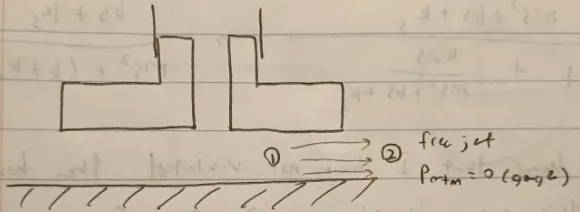
\includegraphics[width=0.6\textwidth]{streamlines.png}
\end{center}
\[p_1 + \frac{1}{2}\rho V_1^2 + \gamma z_1 = p_2 + \frac{1}{2}\rho V_2^2 + \gamma z_2\]
Where:
\begin{itemize}
    \item $z_1 = z_2$
    \item $V_1 = V(r)$
    \item $V_2 = V(R_\text{out})$
    \item $p_1 = p(r)$
    \item $p_2 = p_\text{atm} = 0$ gage
\end{itemize}
Thus the bernoulli equation simplifies to:
\[p(r) = \frac{1}{2}\rho (V(R_\text{out})^2 - V(r)^2)\quad\implies\quad \boxed{p(r)=\frac{\rho Q^2}{8\pi^2 h^2}\left(\frac{1}{R_\text{out}^2} - \frac{1}{r^2}\right), \quad R_1 < r < R_\text{out}}\]
\newpage
\subsection*{Central Jet Region}
\textbf{Define Control Volume and Apply RTT}
\begin{center}
    \includegraphics[width=0.7\textwidth]{central cv.png}
\end{center}
The Reynolds Transport Theorem for conservation of momentum states that the net external force acting on the airflow is equal to the rate of change of momentum of the system, which can be expressed in terms of momentum accumulation within the control volume and net momentum transport across its control surface:
\[\frac{D\vec{P}_\text{sys}}{Dt} = \sum \vec{F}_\text{ext} = \frac{\partial}{\partial t} \int_{C\vol} \rho \vec{V}\, d\vol + \int_{CS} \rho\vec{V}( \vec{V}_\text{rel} \cdot \hat{n}) \, dA\]
For steady incompressible flow within a fixed control volume, the first term is zero since momentum within the control volume does not change (no changes in mass or velocity), and the control volume itself cannot expand to contain more momentum.
\[\implies  \frac{\partial}{\partial t} \int_{C\vol} \rho \vec{V}\, d\vol = 0\]
Expressing the control surface integral as the sum of the momentum fluxes through each of the control surfaces, we have:
\[\sum \vec{F}_\text{ext} = \int_{1} \rho\vec{V}( \vec{V}_\text{rel} \cdot \hat{n}) \, dA
+
\int_{2} \rho\vec{V}( \vec{V}_\text{rel} \cdot \hat{n}) \, dA
+
\int_{3} \rho\vec{V}( \vec{V}_\text{rel} \cdot \hat{n}) \, dA
\]
Term by term:
\begin{itemize}
    \item Surface 1:
    \[
\int_1\rho\vec V(\vec V_{\mathrm{rel}}\cdot\hat n)\,dA=\rho(-V_1\hat k)(-V_1)(\pi R_1^2) = \rho V_1^2\pi R_1^2\hat k
\]
    \item Surface 2:
    \[\int_{2} \rho\vec{V}( \vec{V}_\text{rel} \cdot \hat{n}) \, dA = \int_{2} \rho\vec{V}_2 (V_2) \, dA = \int_{2} \rho V_2^2 \hat{r} \, dA\]
    Assuming constant density and uniform radial velocity magnitude across surface 2, the integral evaluates to zero because the radial unit vectors cancel over the complete cylindrical surface due to axisymmetry.
    \[
\int_2 \rho V_2^2\hat r\,dA=\rho V_2^2R_1h\int_0^{2\pi}\hat r\,d\theta=\vec 0
\]
    \item Surface 3:
    \[\int_{3} \rho\vec{V}( \vec{V}_\text{rel} \cdot \hat{n}) \, dA =0\]
    Since surface 3 is a solid boundary, there is no flow through it and thus no momentum flux.
\end{itemize}
Therefore, the net external force acting on the airflow is:
\[\sum \vec{F}_\text{ext} = \rho V_1^2 \pi R_1^2 \hat{k}\]
Assuming that body forces (gravity) are negligible, the net external force is due to the force from the surface on the airflow AND the force from the pressure at the inlet of the control volume:
\[\vec{F}_{\text{surface on air}} + (-p_1 \pi R_1^2 \hat{k})= \rho V_1^2 \pi R_1^2 \hat{k}\]
\[\implies \vec{F}_{\text{surface on air}} = (\rho V_1^2 \pi R_1^2+p_1 \pi R_1^2) \hat{k}\]
Where $p_1$ is the gage pressure at the central nozzle exit, or the control volume inlet.\\\\
By Newton's third law, the force on the surface due to the airflow is equal in magnitude and opposite in direction:
\[\implies \vec{F}_{\text{air on surface}} = -(\rho V_1^2 \pi R_1^2+p_1 \pi R_1^2) \hat{k}\]
\textbf{Finding $V_1$ using Continuity}\\
For a single inlet, single outlet nozzle with steady, incompressible flow, the volumetric flow rate is constant across any cross-section of the nozzle. Assuming $V_1$ is the average velocity at the nozzle exit:
\[Q_\text{in} = Q_\text{out}\]
\[\implies Q = V_1 (\pi R_1^2)\]
Substituting this into the expression for the force on the surface, we have:
\[
\vec{F}_{\text{air on surface}} = -\left(\frac{\rho Q^2}{\pi R_1^2} + p_1 \pi R_1^2\right) \hat k
\]
\textbf{Finding $p_1$ using Bernoulli}\\
We are given that pressure at the inlet is $p_\text{in} = 15$ cm H$_20$.
\begin{center}
    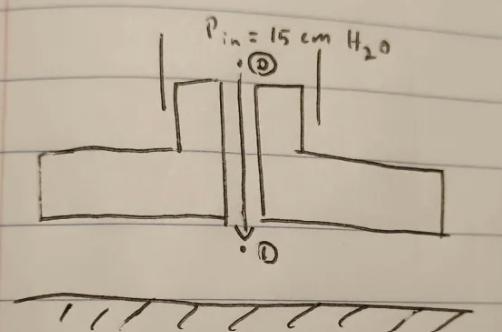
\includegraphics[width=0.4\textwidth]{p1 streamlines.png}
\end{center}
\[
p_0+\frac12\rho V_0^2+\gamma z_0=p_1+\frac12\rho V_1^2+\gamma z_1
\]
Neglecting elevation changes $z_0\approx z_1$, apply continuity:
\[
V_0=\frac{Q}{\pi R_{\mathrm{in}}^2},\qquad V_1=\frac{Q}{\pi R_1^2}
\]
\[
\boxed{p_1=p_0+\frac{\rho Q^2}{2\pi^2}\left(\frac{1}{R_{\mathrm{in}}^4}-\frac{1}{R_1^4}\right)}
\]
\subsection*{Net Force on Surface}
The net force on the surface is the sum of the forces from the central jet region and the annular gap region:
\[\vec{F}_{\text{net}} = \vec{F}_{\text{central}} + \vec{F}_{\text{annular}}\]
Where:
\begin{itemize}
    \item The force from the central jet region is:
    \[\vec{F}_{\text{central}} = \left(-\frac{\rho Q^2}{\pi R_1^2} - p_1 \pi R_1^2\right) \hat k\]
    \item The force from the annular gap region is obtained by integrating the pressure distribution over the area of the annular gap.\\\\
    The net pressure force on the surface (surrounded by $p_\text{atm}$) is where positive $z$ is upward:
    \[d\vec{F} = (p_\text{atm}-p(r))\hat{k}\,dA\]
    Thus for gage pressure, the net force is:
    \[\int d\vec{F} = \int_{R_1}^{R_{\mathrm{out}}} (0-p(r))\hat{k}\,dA\]

\begin{align*}
\vec F_{\mathrm{annular}}
&=-\int_{R_1}^{R_{\mathrm{out}}}p(r)\,2\pi r\,dr\,\hat k\\
&=-\int_{R_1}^{R_{\mathrm{out}}}\frac{\rho Q^2}{8\pi^2h^2}
\left(\frac{1}{R_{\mathrm{out}}^2}-\frac{1}{r^2}\right)2\pi r\,dr\,\hat k =-\frac{\rho Q^2}{4\pi h^2}\int_{R_1}^{R_{\mathrm{out}}}\left(\frac{r}{R_{\mathrm{out}}^2}-\frac{1}{r}\right)dr\,\hat k\\
&=-\frac{\rho Q^2}{4\pi h^2}
\left[\frac{r^2}{2R_{\mathrm{out}}^2}-\ln r\right]_{R_1}^{R_{\mathrm{out}}}\hat k\\
&=\frac{\rho Q^2}{4\pi h^2}
\left[\ln\left(\frac{R_{\mathrm{out}}}{R_1}\right)
-\frac{R_{\mathrm{out}}^2-R_1^2}{2R_{\mathrm{out}}^2}\right]\hat k
\end{align*}
\end{itemize}
\textbf{Putting it all together:}
\[\boxed{\vec F_{\mathrm{net}} = \left(-\frac{\rho Q^2}{\pi R_1^2} - p_1 \pi R_1^2+ \frac{\rho Q^2}{4\pi h^2}\left[\ln\left(\frac{R_{\mathrm{out}}}{R_1}\right) - \frac{R_{\mathrm{out}}^2-R_1^2}{2R_{\mathrm{out}}^2}\right]\right)\hat k}\]
Where $p_1$ is given by:
\[
\boxed{p_1=p_0+\frac{\rho Q^2}{2\pi^2}\left(\frac{1}{R_{\mathrm{in}}^4}-\frac{1}{R_1^4}\right)}
\]
This is valid for steady, incompressible, and inviscid flow, and assumes that the flow is axisymmetric.\\\\
Now, we would have an equation for lift in terms of only geometry and flow rate.
\newpage
\hl{Note (consistency check):} The equation for $p_1$ and the derived equation for $p(r)$ in the annular gap do not agree at $r=R_1$. This is because the model treats the central jet and annular gap as two separate flow regions, without accounting for the transition where the airflow strikes the surface and turns radially outward. Therefore, the pressure distributions are not necessarily continuous at this boundary in our simplified model.
\[p_1=p_0+\frac{\rho Q^2}{2\pi^2}\left(\frac{1}{R_{\mathrm{in}}^4}-\frac{1}{R_1^4}\right)\]
\[p(R_1)=\frac{\rho Q^2}{8\pi^2 h^2}\left(\frac{1}{R_\text{out}^2} - \frac{1}{R_1^2}\right)\]
\begin{center}
    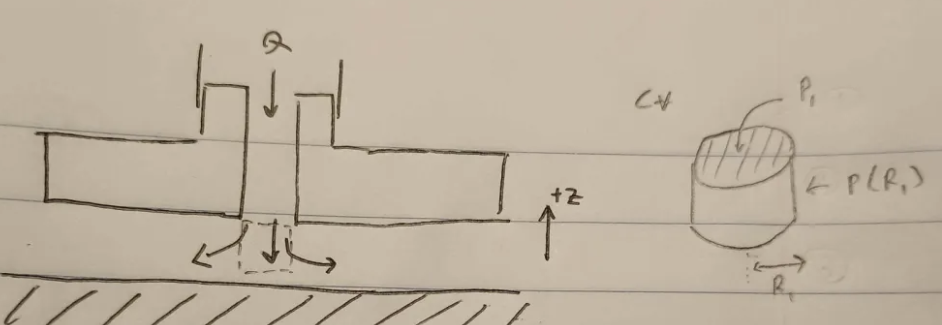
\includegraphics[width = 0.8\textwidth]{inconsistency.png}
\end{center}


\end{document}
